\section{The LUX-ZEPLIN Detector}
\label{sec:lz_detector}
\par
The LUX-ZEPLIN (LZ) experiment is a second-generation direct detection dark matter experiment, named from its predecessor LUX \cite{lux_ref}, and the ZEPLIN series of experiments which pioneered xenon phase detectors \cite{zeplin_3_ref}\footnote{Out of interest for the reader, the full name of the LUX-ZEPLIN experiment can be considered as: "Large Underground Xenon - ZonEd Proportional scintillation in LIquid Noble gases"}.
The LZ experiment is hosted at the Sanford Underground Research Facility (South Dakota, USA), at the 4850 level underground\footnote{4850-feet underground}.

\par
The LZ experiment is a multi-detector system which work together to increase the sensitivity to dark matter candidates.
LZ is comprised of three discrete detectors: a TPC, and two active veto-detectors.
A diagram of the detector systems is shown in \autoref{fig:LZ_Cut_CAD}.

\begin{figure}
    \centering
    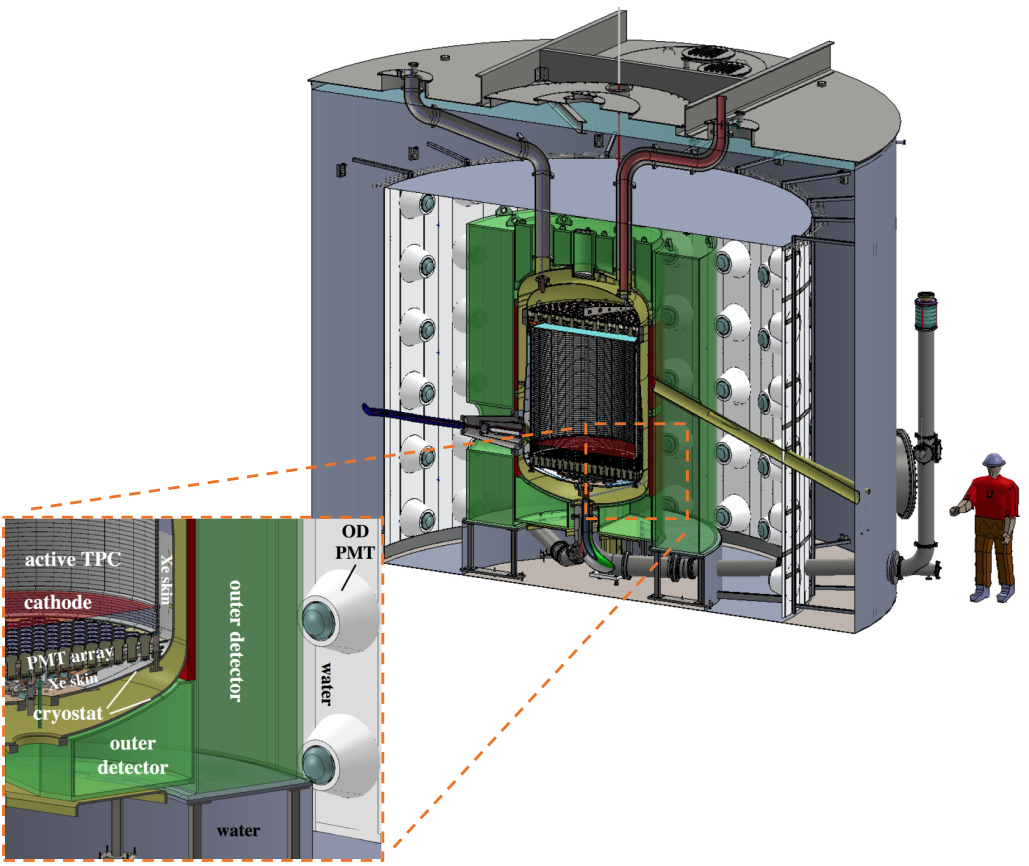
\includegraphics[width=\textwidth]{Figures/LZ/LZ_CAD_with_interactions.png}
    \caption{A schematic of the LZ detector systems as described in the Technical Design Review \cite{LZ_TechnicalDesignReview_ref}.
             Figure from \cite{LZ_TechnicalDesignReview_ref} using adaptation from \cite{LZ_Ibles_LZStats_Thesis_ref}.}
    \label{fig:LZ_Cut_CAD}
\end{figure}

\par
During the course of this thesis, the construction of the LZ experiment was completed, followed by a successful commissioning and calibration phase.
The first Science Run (SR1) concluded in April 2022, with the first result for the WIMP search announced in July 2022.
At the time of writing, the detector is undergoing Pre-SR2 upgrades, with SR2 due to commence in November 2022.

\par
In the remainder of this chapter, the design and construction of the LZ experiment are detailed, with particular emphasis on the TPC and OD, which are relevant for the remainder of this thesis. 
The full design is detailed in the Technical Design Review (TDR) \cite{LZ_TechnicalDesignReview_ref}.

\subsection{Time Projection Chamber}
\label{sec:lz_tpc}
\par
At the core of LZ is a dual-phase (liquid and gas) xenon TPC.
The schematic of the LZ TPC is shown in \autoref{fig:lz_tpc_schematic}.
Photons which are emitted inside of the TPC are detected by 494 Hamamatsu R11410-22 3-inch diameter PMTs, arranged into two arrays.
The first array contains 253 PMTs and is located at the top of the TPC in the GXe, looking down.
The second array, containing 241 PMTs and located at the bottom is immersed in the LXe looking up.
These PMTs were selected as they were developed with low levels of radioactivity and a high quantum efficiency at wavelengths around 175 nm, the characteristic emission of LXe scintillation.
The arrangement of these PMT arrays is not identical, with the bottom array optimised for light collection of S1 signals and the top array optimised for position reconstruction of S2 signals.
\par
The TPC contains three electrodes: a cathode at the bottom, a gate below the liquid surface and an anode in the gas phase, each of which are woven mesh grids \cite{lz_grids_ref}.
The walls of the TPC are enclosed by titanium rings encased in polytetrafluoroethylene (PTFE) panels - a highly reflective material (in excess of 97.3\% in LXe \cite{ptfe_lxe_reflectivity_ref}).
The titanium rings are connected by a ladder of resistors.
These titanium rings shape the electric field, creating a vertical field across the active region so that any charge created in the active region will drift upwards through the liquid to the electroluminescence region.
\par
The TPC active region, which is defined as the volume between the cathode grid and the gate grid, is a cylinder of 1.46m in diameter and height that contains 7 tonnes of Liquid Xenon.
This active region is a significant size increase compared to previous generation detectors such as LUX (250 kg) \cite{lux_ref}, XENON1T (2.2 tonne) \cite{xenon1t_ref} and PandaX (500 kg) \cite{pandax_ref}.
Other current generation xenon TPC experiments include PandaX-4T (3.7 tonne) \cite{pandax_4t_ref} and XENONnT (5.9 tonne) \cite{xenonnt_projected_sensitivty_ref}, with both having recently published results from first runs \cite{pandax_4t_sr1_ref,xenonnt_sr1_er_ref}. 
\par
The electroluminescence region is defined as the distance from the surface of the LXe to the anode grid, a distance of 8 mm.
The distance between the gate grid and the anode grid is 13 mm.
In this region, the electric field can reach 10 kV/cm.
This is typically referred to as the extraction field.
The electric field in the active region can reach 310 V/cm when applying an operating voltage of -50 keV to the cathode.
\par
Below the cathode is a fourth grid which acts to shield the bottom array PMTs from the electric field.
Between this grid and the cathode is a reverse-field region (RFR), where the ionisation from interactions cannot be detected.


\begin{sidewaysfigure}
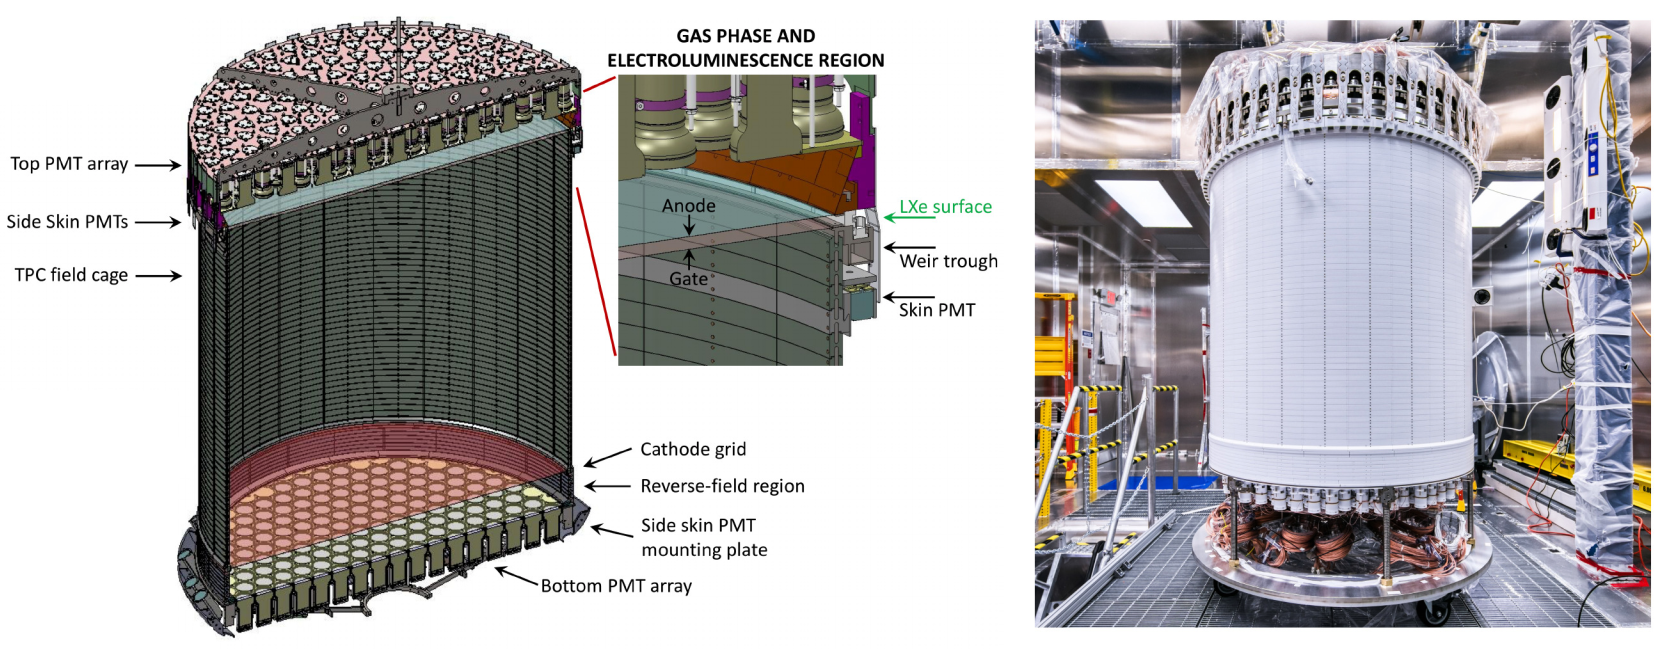
\includegraphics[width=\columnwidth]{Figures/LZ/lz_tpc_schematic.png}%
\caption{Depiction of the LZ TPC detector.
         \textbf{Left:} A schematic drawing of the proposed TPC design for LZ \cite{LZ_TechnicalDesignReview_ref}.
         \textbf{Right:} Photograph of the fully assembled TPC.
}
\label{fig:lz_tpc_schematic}
\end{sidewaysfigure}


\subsection{Veto Detectors}
\label{sec:lz_veto_detectors}
\par
In addition to the TPC, the LZ experiment makes use of two additional detectors.
Neither of these are designed to directly detect dark matter but rather to improve the sensitivity of the TPC by identifying and vetoing events which would otherwise impact the ability to detect dark matter.
Dark matter will scatter once in the TPC and then leave the experiment.
Other backgrounds may also only scatter once in the TPC but have a high probability of scattering in one of the veto detectors and can therefore be vetoed.
The veto operating principle is shown in \autoref{fig:LZ_Veto_Principle}.

\par
Firstly, surrounding the TPC is a layer of LXe referred to as the xenon skin, or Skin detector.
This region of LXe has to exist due to the geometrical challenge of placing the TPC inside of a cryovessel.
It is made active by 38 Hamamatsu R8778 2-inch PMTs in the barrel and bottom dome and 93 R8520 1-inch PMTs in the top barrel region.
Similarly to the TPC, the inner wall of the cryostat is coated with PTFE, but is optically de-coupled from the TPC.
It is designed primarily to veto $\gamma$ events.

\par
Outside of the cryostat is the second veto detector, the Outer Detector (OD).
This is made up of a number of acrylic tanks which contain a liquid scintillator doped with gadolinium (GdLS).
Together these provide near 4$\pi$ coverage around the TPC and act to identify neutron interactions.
The OD is described in more detail in Chapter \ref{chapter:lz_outer_detector}.

\begin{figure}
    \centering
    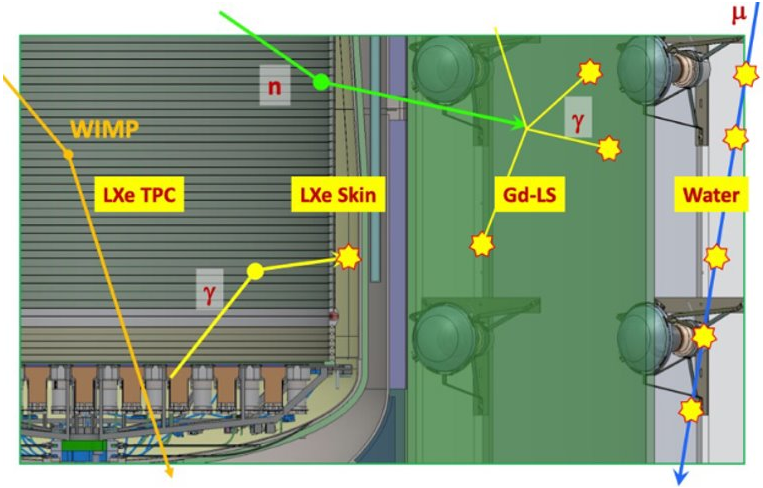
\includegraphics[width=0.75\textwidth]{Figures/LZ/lz_veto_plan.png}
    \caption{Depiction of the operating principle of the veto detectors and the particles that they are designed to veto.}
    \label{fig:LZ_Veto_Principle}
\end{figure}


\subsection{Calibrations}
\label{sec:lz_calibrations}
\par
In order for the experiment to work and have understandable results, a set of calibrations are conducted to characterise the energy scale, energy threshold and photon detection efficiency.
LZ has a large variety of sources available which are able to characterise each detector.
A summary of the sources used for commissioning and the first science run (SR1) is shown in \autoref{tab:LZ_Used_Calibration_Sources}.
Additional sources available to LZ are outlined in the LZ Technical Design Review \cite{LZ_TechnicalDesignReview_ref}.
\par
Radioactive impurities within the xenon are evenly distributed through the TPC detector volume.
These are used to model the position reconstruction, $G_1$ and $G_2$ of the TPC, as well as the energy scale.
As the Skin detector contains the same xenon and, therefore, the same sources, they can be used for the Skin position reconstruction and energy scale.
In addition to the naturally occurring impurities, other sources can be injected into the xenon via the circulation system \cite{christophernedlik_thesis_ref}.
\par
Beyond the internal and injected sources, a suite of external sources are also used.
These are deployed in calibration source deployment tubes (CSD) which run into the cryostat allowing the OD to be bypassed.
These sources are used primarily for energy calibration of all three detectors.
The other external sources external to the TPC are neutron generators which are deployed in a unique fashion.
For $^{88}$YBe deployment, an OD tank is removed and replaced by the source.
Deuterium-deuterium (DD) is deployed externally to the water tank. 
It is a directional source with neutrons directed through a calibration tube that extends through the OD acrylic tanks to the OCV.

\begin{table}
    \centering
    \begin{tabular}{c|c|c|c}
    \hline
    Isotope       & Interacting particle         & Purpose                    & Deployment \\
    \hline
    ${}^{83m}$Kr  & beta/gamma, 32.1 keV/9.4 keV & TPC (x,y,z)                & Internal  \\
    ${}^{131m}$Xe & 164 keV gamma                & TPC (x,y,z), Xe skin       & Internal  \\ 
    ${}^{220}$Rn  & various alphas               & xenon skin                 & Internal  \\
    ${}^{220}$Rn  & various alphas               & ER band                    & Internal  \\
    Tritium       & beta                         & ER band                    & Injected  \\
    AmLi          & (alpha, n)                   & NR band                    & CSD       \\
    ${}^{252}$Cf  & spontaneous fission          & NR efficiency              & CSD       \\
    ${}^{57}$Co   & 122 keV gamma                & Xe skin threshold          & CSD       \\
    ${}^{228}$Th  & 2.615 MeV gamma              & OD energy scale            & CSD       \\
    ${}^{22}$Na   & back-to-back 511 keV gamma’s & TPC and OD sync            & CSD       \\
    ${}^{88}$YBe  & 152 keV neutron low-energy   & NR response                & External  \\
    DD            & 272 keV and 2,450 keV neutron & NR light and charge yields & External 
    \end{tabular}
    \caption{LZ calibration sources that were used for calibration prior to the first science run along with the calibration purpose and deployment method. Table populated with information from \cite{LZ_TechnicalDesignReview_ref}.}
    \label{tab:LZ_Used_Calibration_Sources}
\end{table}


\subsection{Backgrounds}
\label{sec:lz_backgrounds}
\par
As previously discussed, the direct detection dark matter search philosophy is to search for an excess in nuclear recoils.
In order for this to be achievable, a deep understanding of the backgrounds that are expected is required.
In this section, the dominant backgrounds expected in the TPC are discussed.

\par
The first set of backgrounds are from detector components.
Given that the detector has to be made of something, there is no getting away from the fact that this will contribute to the recoils detected.
As this can be a limiting factor for sensitivity to dark matter, LZ undertook a comprehensive screening campaign prior to construction \cite{LZ_assay_ref}.
In addition to radioactivity embedded within the detector materials, there is also surface contamination.
The greatest contribution to this is from plate-out of ${}^{222}$Rn progeny as well as any dust on the detector.
The frequent $\alpha$-decays within the decay chain also lead to ($\alpha$,$n$) reactions.
These are the most dangerous backgrounds as they are NR events and indistinguishable from a dark matter scatter in the TPC.
To reduce the levels of surface contamination introduced during detector assembly, the TPC was assembled in a radon-reduced clean room\footnote{better than a class 1000 cleanroom.} with extensive UV inspections to ensure that the dust levels were kept to a minimum.

\par
The environment in which the detector is placed also contributes to the background rate.
The $\gamma$-flux from the cavern where the detector is placed is the largest contributor to this category \cite{LZ_Gamma_Ray_Background_ref}.
The origins of these $\gamma$-rays are detailed in the following chapter.
Other contributions are from radioactive isotopes created by exposure to cosmic rays on the Earth's surface.
Of particular note are $^{127}$Xe and ${}^{37}$Ar from activation of xenon \cite{lux_xenon_activation_ref,lz_argon37_ref}, and $^{46}$Sc from activation of titanium \cite{LZ_TechnicalDesignReview_ref}.
All of the aforementioned backgrounds are able to be removed to some degree by analysis cuts.

\par
Within the LXe a number of radioactive isotopes will be dispersed.
Of particular note are $^{222}$Rn progeny, $^{220}$Rn progeny, $^{85}$Kr and $^{39}$Ar.
All of these are $\beta$-decays at low energies, increasing the rate of ER events.
At higher energies, both $^{222}$Rn and $^{220}$Rn have $\alpha$ decays and $\gamma$ excitation as well.
Gas charcoal chromatography was used to remove $^{85}$Kr and $^{39}$Ar from the xenon prior to being circulated through the detector \cite{xenon_prufication_chromatography_ref}.
The xenon is constantly circulated in the detector, during which time radon is removed \cite{marisarthurs_thesis_ref}.

\par
$\gamma$s from any of the aforementioned backgrounds have the potential to scatter multiple times but with a suppressed S2 signal.
These events are referred to as $\gamma$-X.
A $\gamma$-X event occurs typically when there is a scatter in the RFR followed by a scatter in the active region.
As there are two scatters, the S1 size is enhanced.
However, only the contribution from the second scatter will result in an S2.
The resultant interactions appear as a single scatter with a larger S1 than a typical ER event.
These appear as ER events which leak into the NR band.


\par
Finally, there are astrophysical backgrounds from neutrinos, an irreducible background.%, not removable by any analysis cut.
These contribute to the ER background via neutrino-electron scattering and to the NR background via neutrino-nucleus scattering.
Electron recoils are caused by solar neutrinos primarily from the $pp$ solar chain \cite{solar_neutrinos_ref}.
Nuclear recoil neutrinos fall into two categories: low energy recoils from solar neutrinos ($^{8}$B and $hep$) and high energy recoils from atmospheric and diffuse supernova neutrinos (DSN).

\par
There are far more ER backgrounds than NR backgrounds.
As a WIMP scatter is an NR event, each NR background is much more important than any ER background assuming that there is good separation between recoil types.

\subsection{Analysis Cuts}
\label{sec:lz_analysis_cuts}
\par
As indicated, some of the backgrounds can be reduced by analysis cuts. 
The core cuts for searching for an excess of recoils in LZ are listed below.
\begin{itemize}
    \item \textbf{SS}: Select events which have only scattered once, ``single scatter". This refers to the particle which sets off the cascade seen in \autoref{fig:er_nr_tracks}. Particles which scatter more than once are not compatible with dark matter as their likelihood to scatter twice is too low. This cut is defined as events which have a single S1 pulse and a single S2 pulse in the event.
    \item \textbf{FID}: Removal of events where reconstruction of energy is poor and to incorporate LXe self-shielding. This cut is applied on the reconstructed \{$x,y,z$\} of a scatter to select events in an inner region of the TPC LXe. Decays originating from the detector components are suppressed in this way.
    \item \textbf{ROI}: Select events where the recoil energy is in the range expected from a WIMP scatter. Typically this is between 1.65-6.5 keV ER events and 6-30 keV NR events. For other dark matter models, such as EFT searches this requirement changes.% This cut is applied on the S1 pulse size not energy.
    \item \textbf{Veto}: Remove events which are inconsistent with dark matter due to scattering more than once. This removes both neutrons and $\gamma$s. The veto detectors work as anti-coincidence detectors so an event is vetoed if the Skin or OD saw a pulse within some time window of the S1 in the TPC.
\end{itemize}
In data taking, additional cuts are often required to account for experimental features not anticipated in simulations.
As such, the above list should be considered as a ``core" selection, with a requirement of data-driven cuts potentially required later.

\subsection{Dark Matter Search Strategy}
\par
The primary direct dark matter search strategy of LZ is to search for an excess in NR events.
In order to do this, an event needs to be defined and recorded, and ultimately the pulses which are output from the PMTs need to be reconstructed.
The planned approach is detailed in \cite{LZ_TechnicalDesignReview_ref}, with the approach adopted for the first data run detailed in \cite{lz_ws_sr1_ref}.

\par
An event is defined simply as a window of time in which the output from all PMTs is saved, typically for LZ this is 4 ms in length.
LZ utilises a number of different triggers to determine when data should be recorded, utilising the logic based upon \cite{lux_trigger_logic_ref}, with application to LZ detailed in \cite{nicolasangelides_thesis_ref}.
From the trigger activation, a period of time before and after the trigger is recorded.
The two triggers of relevance to this thesis are briefly discussed below.

\paragraph{S2 Trigger}
\par
This is the primary dark matter search trigger.
Tuned to trigger on a large pulse in the TPC that is in line with what is expected from an S2 pulse.
The S1 pulse will reside within the pre-trigger time window.
The veto detectors search the post-trigger window for $\gamma$ and neutron events.

\paragraph{Random Trigger}
Often referred to as the ``heartbeat trigger", data is recorded at fixed time intervals.
It can act as a measurement of backgrounds as it is a fixed amount of data recorded periodically.

\par
On data which passes the analysis cuts, a statistical analysis is performed.
A multidimensional Profile Likelihood Ratio (PLR) fit is used to probe how well a background-only model vs a background and WIMP signal model fit to the data.
In both projected sensitivity and SR1 studies, LZ has limited this to two dimensions, \{S1$_c$, log$_{10}$S2$_c$\}.
However, future analysis will extend this to include \{$x,y,z$\} as has been done in previous TPC experiments \cite{LUX_RUN1_EFT_2021,LUX_RUN4_EFT_2021,shaunalsum_thesis_ref}.
A full description of the PLR used for the WIMP sensitivity projections and SR1 can be found in \cite{LZ_Ibles_LZStats_Thesis_ref}. 
A detailed description of the application to LZ monte-carlo data generated prior to SR1 is described in \cite{jonathannikoleyczik_thesis_ref}.

\subsection{Simulations}
\label{sec:lz_simluations_chain}
\par
The models used to fit to data come from simulations of signal and background processes.
Additionally, these simulations influenced the design and construction of the experiment.
A brief overview of the simulation chain is given below and in \autoref{fig:lz_simulation_chain}.
A more thorough explanation is available in \cite{lz_simulations_ref} and \cite{theresafruth_thesis_ref}.
\par
The primary simulation package used by LZ is called BACCARAT\footnote{The acronym comes from, \textbf{B}asically \textbf{A} \textbf{C}omponent-\textbf{C}entric \textbf{A}nalog \textbf{R}esponse to \textbf{A}ny\textbf{T}hing.}.
BACCARAT is used to simulate particle interactions built upon the GEANT4 simulation package \cite{geant4_geometry_ref}.
Inside BACCARAT, the LZ experiment is built as a detector geometry.
From a simulation of a particle, interactions and energy deposits are recorded.
If the deposit occurred within the xenon volume, the Noble Element Simulation Technique (NEST) is used to convert the deposit into scintillation photons, and ionisation electrons \cite{nest_1_ref}.
There are two running modes for BACCARAT: energy deposits only and optical photon propagation.
If energy deposit-only simulations are run, then the output is run through a detector model response, LZLAMA.
In the detector model response, the energy deposits are converted into reconstructed quantities, such as S1$_c$ and log$_{10}$(S2$_c$), which characterise an event.
The detector model response is informed by both data and optical photon simulations.
\par
If optical photon propagation simulations are used, then individual photons are propagated and recorded if they reach a PMT.
A photon is considered to be optical when its wavelength is much greater than the typical atomic spacing.
The photons that hit PMTs are converted into waveforms by the Detector Electronics Response (DER) package, which models the PMT response.
The output of the DER should match, or be close to, what is observed in data.
The waveforms are then processed by the same analysis package (LZAP) that the data is processed with, where pulses are found, classified and reconstructed.
The output of this is the same quantities as from LZLAMA.
\par
For example, if the spontaneous fission of Uranium is simulated, originating from a PMT in the TPC, then both the $\gamma$s and neutrons from the fission will be simulated.
These will propagate within BACCARAT and all energy deposits recorded.
Each particle and all secondary particles\footnote{secondary particles are particles produced as a result of the first particle except optical photons.} will be tracked and recorded until all particles are absorbed or until the particle energy is below some energy threshold.
On these energy deposits, depending upon the simulation type this will be the end of the simulation or the optical photons will be generated and propagated.
\begin{figure}
    \centering
    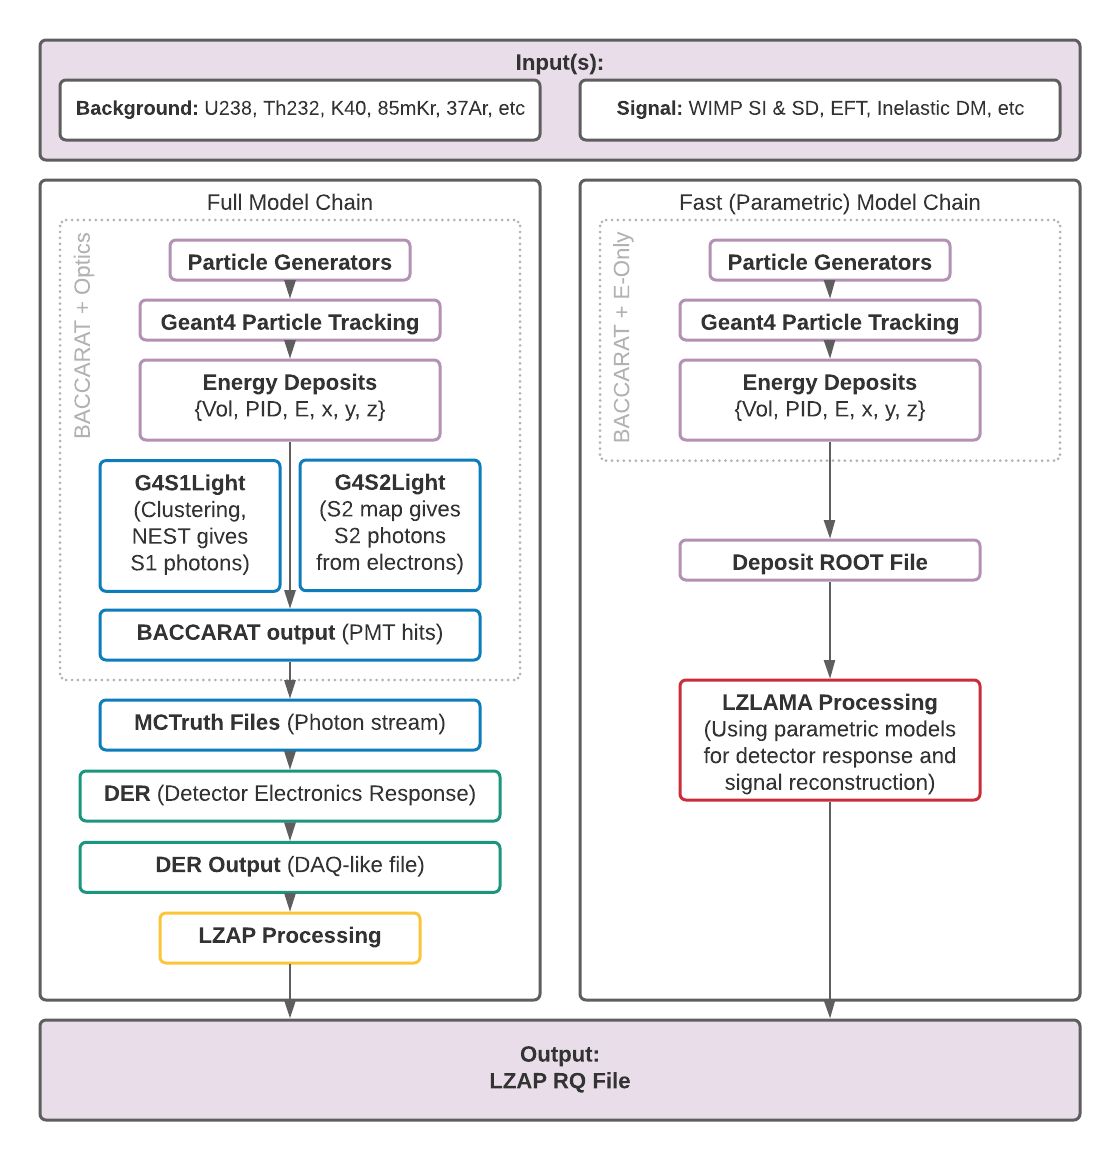
\includegraphics[width=15cm]{Figures/LZ/FullAndFastChains.png}
    \caption{LZ simulation and analysis framework for both the energy deposit-only simulations (fast chain) and optical propagation chain (full chain).
             Image produced by the LZ collaboration.}
    \label{fig:lz_simulation_chain}
\end{figure}







